\documentclass[12pt,a4]{article}
\usepackage[left=1.8cm,right=1.8cm,top=32mm,columnsep=20pt]{geometry}

\usepackage[utf8]{inputenc} %Formato de codificación
\usepackage[spanish, es-tabla, es-nodecimaldot]{babel}
\usepackage{amsmath} %paquete para escribir ecuaciones matemáticas
\usepackage{float} %Para posicionar figuras
\usepackage{graphicx} %Para poder poner figuras
\usepackage{tikz}
\usetikzlibrary{positioning}
\usetikzlibrary{shapes.geometric, decorations.pathreplacing}

\title{Analisis movimiento de un pendulo}
\author{Francisco Carruthers, Facundo Firpo y Joel Jablonski\\ [2mm]
\small \texttt{\{fcarruthers, ffirpo, jjablonski\}@udesa.edu.ar}\\
\small Fisica I, tutorial Vinograd}
\date{2do Semestre 2024}


\begin{document}

\maketitle

\begin{abstract}
    Se investigó el movimiento de un péndulo simple variando la longitud de la cuerda y la masa del péndulo. El objetivo principal fue registrar y caracterizar su trayectoria, determinar el rango angular donde se cumplen las condiciones de pequeñas oscilaciones, calcular la frecuencia de oscilación y estimar la gravedad efectiva. Primero, se mantuvo una longitud fija de cuerda, variando los ángulos iniciales con diferentes masas, y luego se analizó cómo la longitud de la cuerda afecta el movimiento al fijar el ángulo y la masa. La gravedad efectiva obtenida fue de $9.5 \pm 0.6 \text{m/s}^2$. Además, evaluamos la influencia de los parámetros sobre la frecuencia de oscilación ($\omega$) del péndulo, concluyendo que, aunque la masa no altera la frecuencia, la longitud sí lo hace; los valores obtenidos fueron \(0.75 \, \text{s}^{-1}\) para \(42 \, \text{cm}\), \(0.98 \, \text{s}^{-1}\) para \(26 \, \text{cm}\) y \(1.3 \, \text{s}^{-1}\) para \(15 \, \text{cm}\). Finalmente, se identificó el rango de ángulos donde se cumplen pequeñas oscilaciones, siendo de aproximadamente ángulos menores a $25^\circ$.

\end{abstract}

\section{Introducción}

El estudio del péndulo simple ha sido fundamental en la comprensión de la dinámica oscilatoria y los principios físicos básicos que la rigen. A través de este experimento, se analizaron los efectos de variables clave, como el ángulo inicial, la longitud de la cuerda y la masa del péndulo, sobre el periodo de oscilación y la frecuencia angular. La ecuación del periodo de un péndulo simple esta dada por:

\begin{equation}
    T = 2 \pi \sqrt{\frac{L}{g}}
    \label{eq:periodo}
\end{equation}

Esta ecuación asume que el péndulo oscila en el régimen de pequeñas oscilaciones, donde el ángulo de desplazamiento es pequeño y la fuerza restauradora es proporcional al desplazamiento. Donde podemos definir que $sin(\phi) \approx \phi$ para ángulos pequeños. En la practica intentamos verificar esta aproximación y encontrar hasta que $\phi$ se cumple variando los ángulos iniciales y comparando el movimiento con el esperado.

La ecuación \ref{eq:periodo} indica que este es independiente tanto de la masa del péndulo como de su ángulo inicial en el régimen de pequeñas oscilaciones, pero depende de la longitud de la cuerda.

Asimismo, la frecuencia angular \(\omega\) se puede expresar en términos del periodo como:

\begin{equation}
    \omega = \frac{1}{T}
    \label{eq:omega}
\end{equation}

Esto sugiere que sugiere que, al reducir la longitud de la cuerda, la frecuencia angular aumentará, reflejando un ciclo de oscilación más rápido.

A partir de las mediciones obtenidas, buscamos estimar una gravedad efectiva mediante el análisis de la pendiente en la gráfica de \( T^2 \) frente a la longitud \( L \), considerando que esta pendiente corresponde a:
\begin{equation}
    T^2 = \frac{4 \pi^2}{g} L
    \label{eq:gravedad}
\end{equation}

Este enfoque permite no solo una estimación experimental de \( g \), sino también la evaluación de la precisión de nuestro sistema.

\begin{figure}[H]
    \centering
    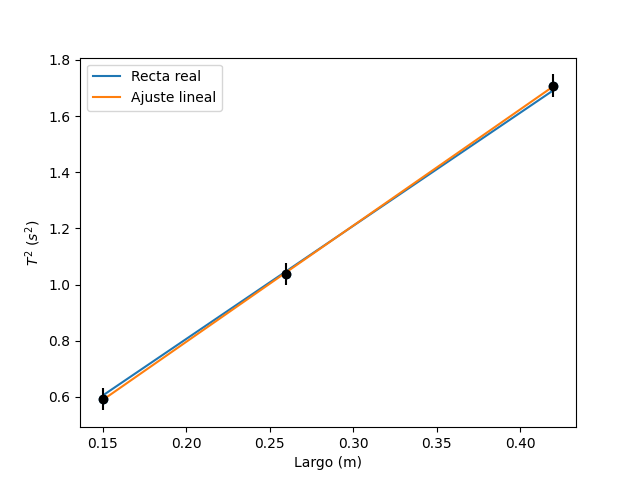
\includegraphics[width=0.6\linewidth]{gravedad.png}
    \caption{Regresión lineal de \( T^2 \) vs \( L \) para estimar la gravedad}   
    \label{fig:gravedad}
\end{figure}

Despejando g de la pendiente de la recta obtenemos: $g = 9.5 \pm 0.6 m/s^2$. Este parámetro incluye a la gravedad real y a los errores de medición del experimento.

Este informe abordará el desarrollo experimental, los métodos de análisis de los datos y la discusión de los resultados, con el fin de proporcionar una comprensión detallada del comportamiento oscilatorio de un péndulo y su relación con los parámetros físicos involucrados.

\section{Practica experimental}

\begin{figure}[H]
    \centering
    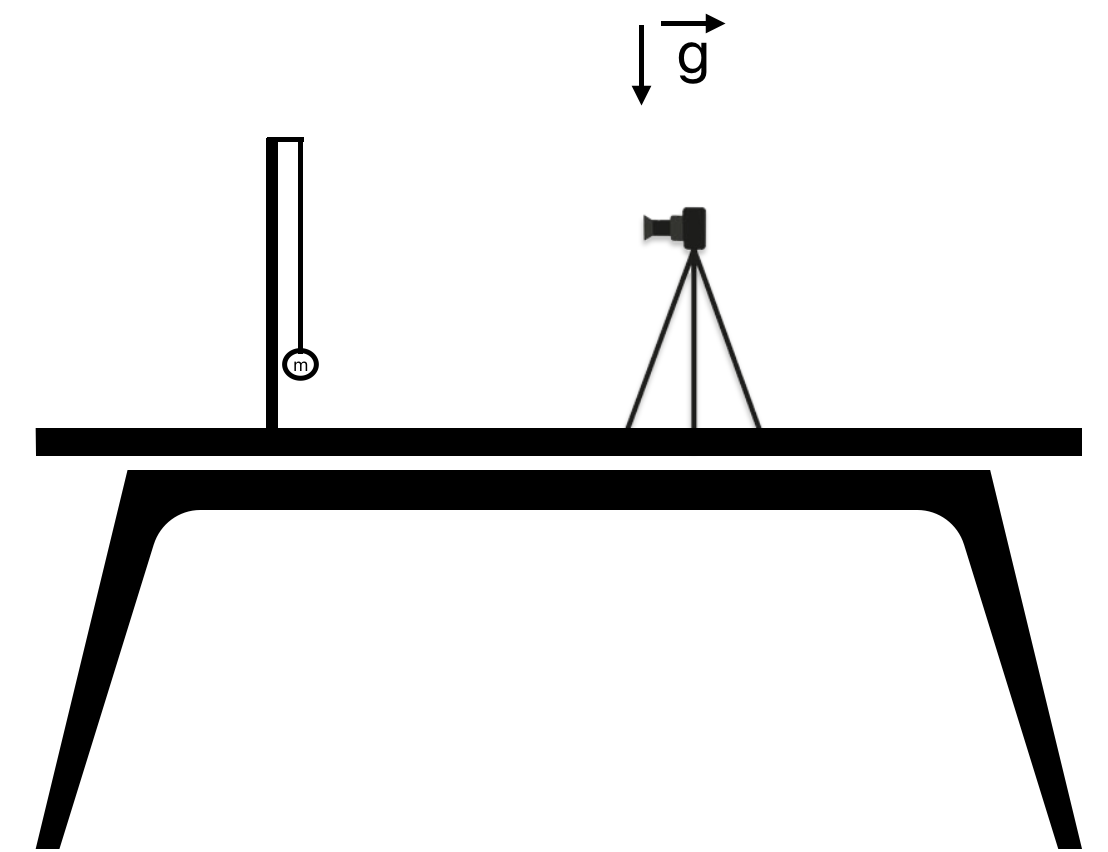
\includegraphics[width=0.6\linewidth]{esquema.png}
    \caption{Esquema del experimento donde m y el largo de la cuerda son variables}   
    \label{fig:esquema}
\end{figure}

Para llevar a cabo el experimento, dispusimos de un sistema compuesto por una masa, una soga y una cámara, que nos permitió construir un péndulo simple y grabar sus movimientos. El esquema del sistema se muestra en la Figura \ref{fig:esquema}. La masa y la longitud de la soga se pueden variar, lo que nos permitió experimentar con diferentes condiciones iniciales y observar sus efectos en el comportamiento del péndulo simple.

Para la adquisición de datos, utilizamos un teléfono para filmar los movimientos del péndulo y posteriormente analizamos los videos con el programa \textit{Tracker}, que permite seguir una masa específica en función del tiempo y registrar su posición en un sistema de coordenadas definido. Para obtener una referencia de distancia, colocamos una cinta métrica en el fondo de cada video, permitiendo al programa calibrar la relación entre píxeles y distancia real y, así, establecer la posición de la masa con precisión.

Una vez construido el sistema, procedimos con el experimento. Primero, mantuvimos una masa constante de $23 \pm 0.1 \, \text{g}$ y una longitud de soga de $42 \pm 0.1 \, \text{cm}$ y variamos los ángulos iniciales, utilizando valores de $\theta = \{55^\circ, 45^\circ, 25^\circ, 15^\circ, 10^\circ\} \pm 1^\circ$. Estos datos nos permitieron analizar el rango angular en el que se cumplen las condiciones de pequeñas oscilaciones, de modo que el péndulo se pueda modelar como un movimiento armónico simple.

Para el siguiente análisis, empleamos un largo fijo de $42 \pm 0.1 \, \text{cm}$, un ángulo inicial de $25^\circ \pm 1^\circ$ y variamos la masa, usando valores de $m = 5 \pm 1 \, \text{g}$, $m = 23 \pm 1 \, \text{g}$ y $m = 72 \pm 1 \, \text{g}$. El objetivo de este experimento fue estudiar el impacto de la masa en la frecuencia de oscilación del péndulo simple. Además, experimentamos manteniendo constantes la masa y el ángulo (con valores de $m = 23 \pm 0.1 \, \text{g}$ y $\theta = 25^\circ \pm 1^\circ$) y variando la longitud de la soga con valores de $L = 42 \pm 0.1 \, \text{cm}$, $L = 26 \pm 0.1 \, \text{cm}$ y $L = 15 \pm 0.1 \, \text{cm}$. Esto nos permitió analizar la dependencia de la frecuencia de oscilación con respecto a la longitud de la soga.

Finalmente, con los datos obtenidos y utilizando las ecuaciones de período y frecuencia del péndulo simple, calculamos la gravedad efectiva.


Los errores que tuvimos en cuenta fueron los siguientes:

\begin{itemize}
    \item Error en la medición del largo de la soga: $\pm 0.1 cm$
    \item Error en la medición del angulo inicial: $\pm 1^\circ$
    \item Error en la posición de la bolita: $\pm 1 cm$ (radio de la bolita)
\end{itemize}

Para medir la soga usamos un metro que tiene marcas cada 0.1 cm por lo que ese es nuestro error. Para el angulo usamos trigonometría y calculamos la distancia del centro del péndulo necesaria para que el angulo sea el deseado, al tener un error de $\pm 1 cm$ en la medición de la distancia, el error en el angulo es de $\pm 1^\circ$. Por ultimo, el error en la posición de la bolita es debido a que el programa \textit{Tracker} no sigue perfectamente el centro de la bolita, por lo que tenemos un error de $\pm 1 cm$ que representa el radio de la bolita.

\section{Seguimiento de la trayectoria}

\begin{minipage}{0.5\textwidth}
    Primero descargamos los videos de los experimentos y los abrimos en el programa \textit{Tracker}. Luego, seleccionamos la masa y seguimos su trayectoria en función del tiempo usando un feature que ofrece la aplicación. El seguimiento lleva un error asociado ya que no sigue perfectamente el centro de la bolita por lo que, en nuestras bolitas de 2cm de diámetro, tenemos un error de $\pm 1cm$. También, definimos un sistema de coordenadas polares con el origen en el inicio de la soga. Para determinar distancias en el video, colocamos una cinta métrica en el fondo de la escena y calibramos el programa para que pueda determinar distancias en el video. 
\end{minipage}
\begin{minipage}{0.5\textwidth}
    \centering
    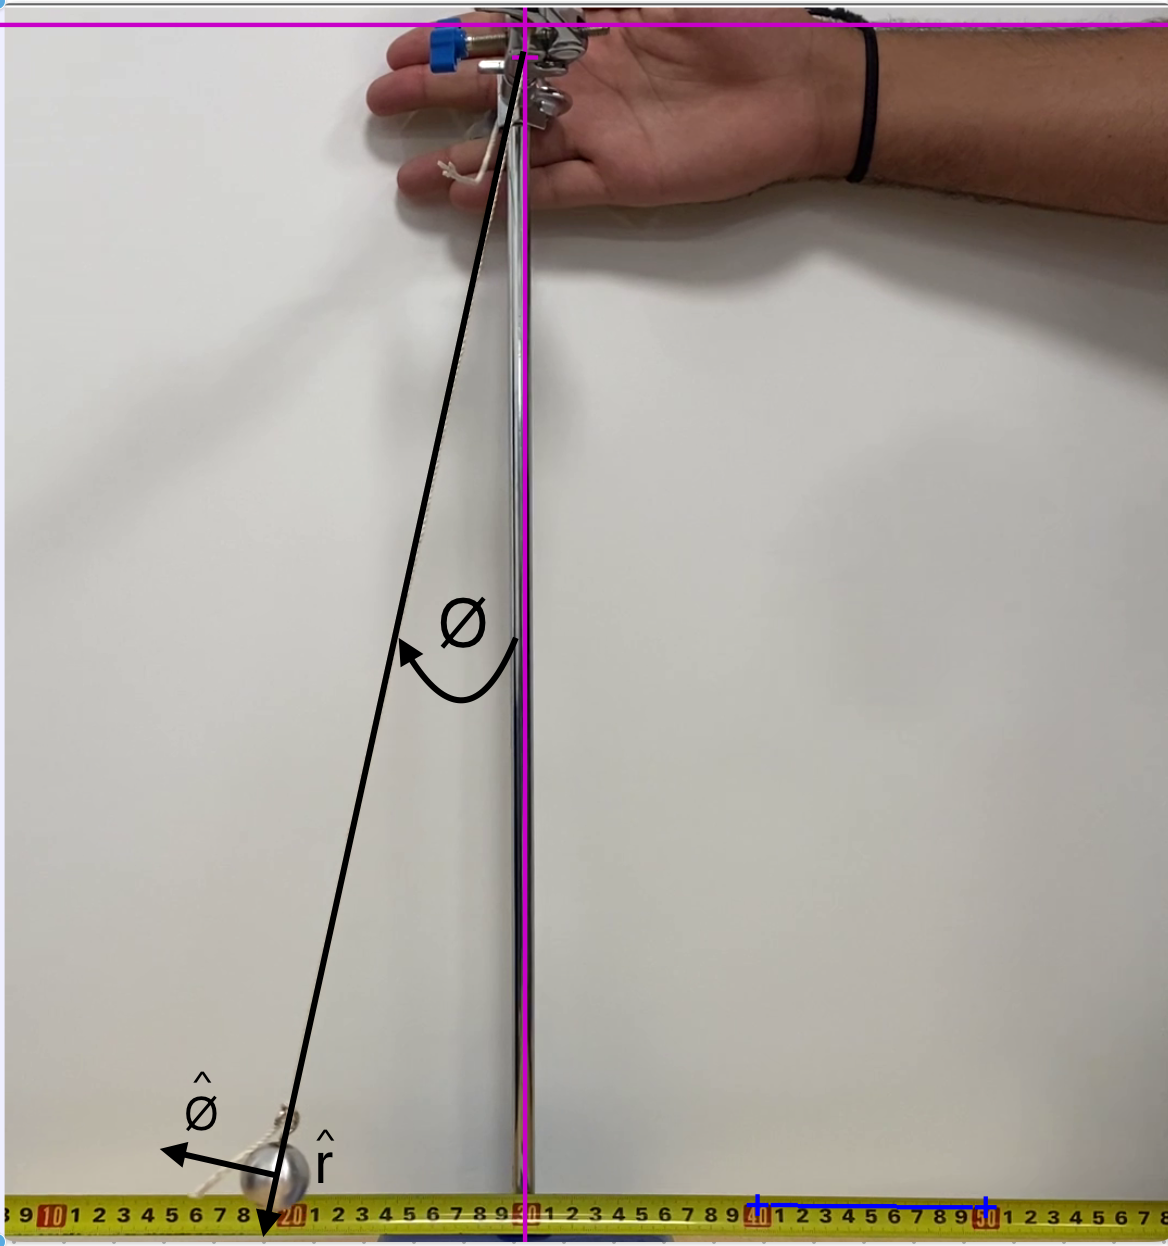
\includegraphics[width=0.8\linewidth]{tracker.png}
\end{minipage}

\newpage

\section{Resultados}

En primer lugar, analizamos la relación entre el periodo de oscilación y la longitud de la soga. Dejando fijos la masa ($23 \pm 1 g$) y el angulo inicial ($25 \pm 1 ^\circ$) obteniendo los siguientes resultados:

\begin{figure}[H]
    \centering
    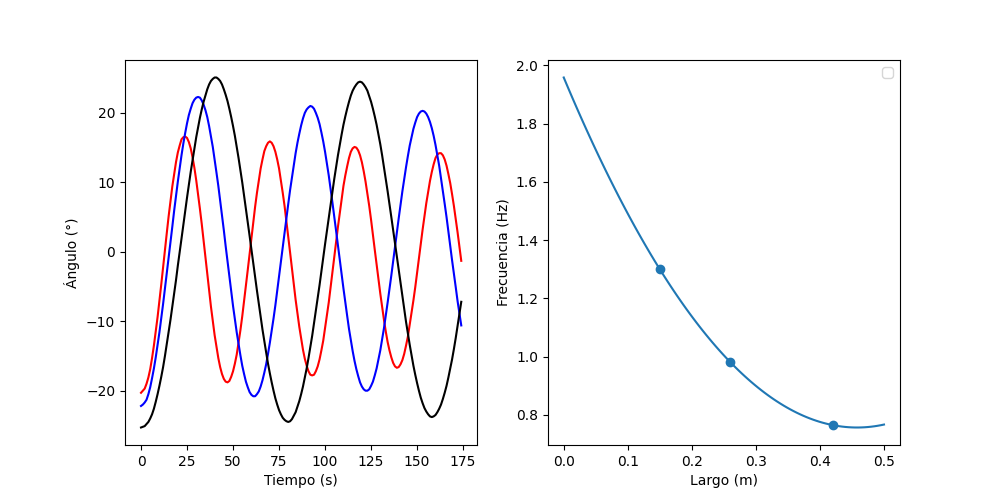
\includegraphics[width=0.6\linewidth]{largo.png}
    \caption{Posición de la masa en función del tiempo para distintos largos de soga}
    \label{fig:largo}
\end{figure}

Se puede observar como el largo de la soga afecta la frecuencia del movimiento. A mayor largo, menor frecuencia. Esto se debe a que la bolita recorre una mayor distancia. Sabemos que la longitud de arco esta definida como $d = r \theta$, por lo que a mayor longitud de soga, mayor longitud de arco recorre la bolita.

\begin{figure}[H]
    \centering
    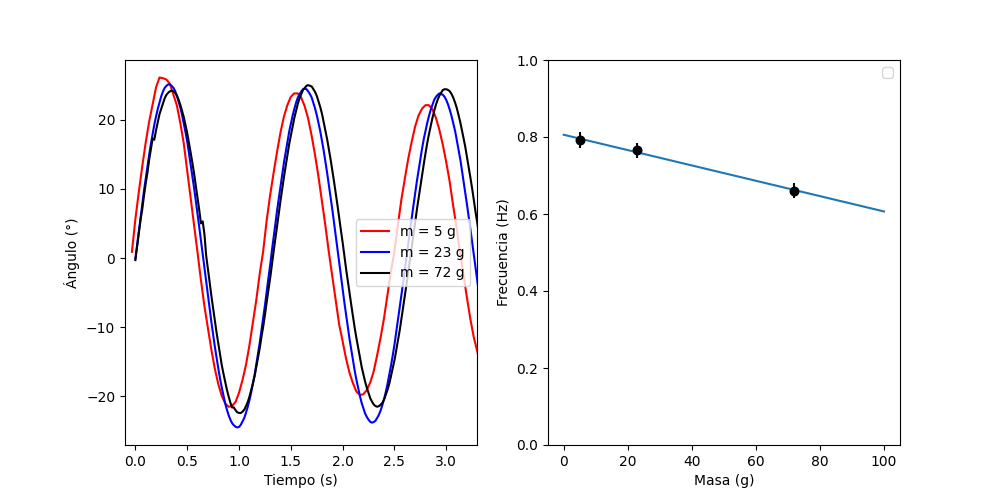
\includegraphics[width=0.6\linewidth]{peso.png}
    \caption{Posición de la masa en función del tiempo para distintas masas}
    \label{fig:masa}
\end{figure}

Se puede observar como la masa de la bolita no afecta la frecuencia del movimiento excepto cuando la masa es chica. Esto se debe a en el experimento la soga no es perfectamente rígida, por lo que, al tener poca masa, el movimiento de la soga se deforma.

Luego, variamos los ángulos iniciales dejando fijo la masa ($23 \pm 1 g$) y largo de la soga ($42 \pm 0.1 cm$) para poder analizar la suposición de pequeñas oscilaciones. Para los distintos ángulos iniciales se obtuvieron los siguientes resultados:

\begin{figure}[H]
    \centering
    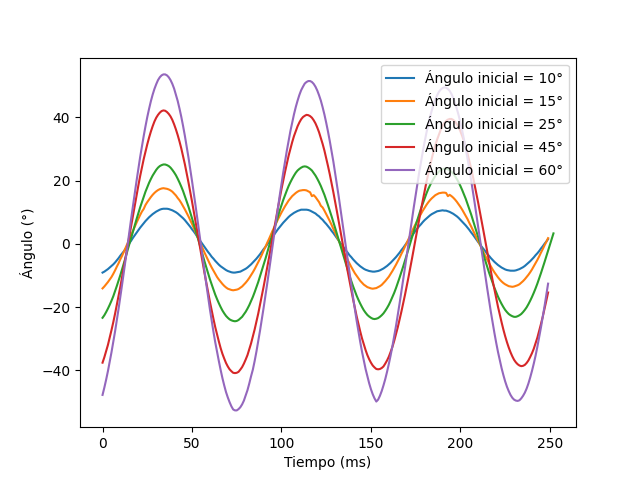
\includegraphics[width=0.6\linewidth]{angulos.png}
    \caption{Posición de la masa en función del tiempo para distintos ángulos iniciales}
    \label{fig:angulos}
\end{figure}

Se puede observar como la amplitud del movimiento no afecta la frecuencia del mismo.

Para determinar el rango de ángulos en el cual se cumple la aproximación de pequeñas oscilaciones en el péndulo, calculamos el error cuadrático medio (ECM) entre las trayectorias experimentales medidas y las trayectorias obtenidas mediante la aproximación lineal. 

\[
\text{ECM} = \frac{1}{n} \sum_{i=1}^{n} (y_i - \hat{y}_i)^2
\]

Donde $y_i$ es la posición de la masa en el tiempo $i$ medida experimentalmente y $\hat{y}_i$ es la posición de la masa en el tiempo $i$ calculada mediante la aproximación de pequeñas oscilaciones.

El valor del ECM se presenta en la Figura \ref{fig:pequeñas_oscilaciones}, donde se observa cómo varía con el ángulo inicial.

\begin{figure}[H]
    \centering
    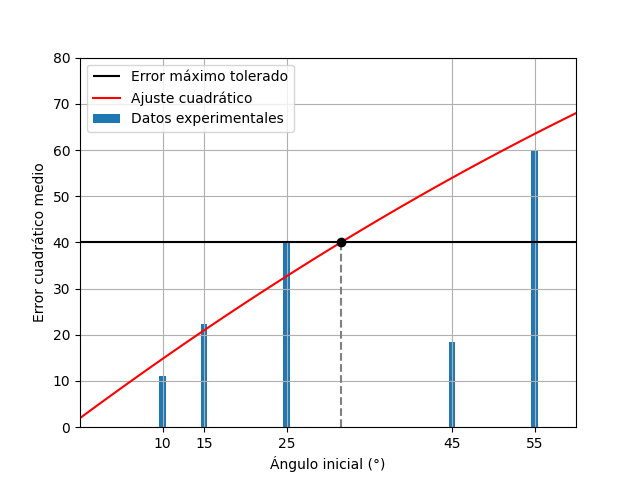
\includegraphics[width=0.6\linewidth]{peq_oscilaciones.png}
    \caption{Error cuadrático medio bajo la aproximación de pequeñas oscilaciones.}
    \label{fig:pequeñas_oscilaciones}
\end{figure}

Observando el gráfico de la Figura \ref{fig:pequeñas_oscilaciones}, determinamos que la aproximación de pequeñas oscilaciones es válida hasta aproximadamente $25^\circ$, una observación que tuvimos sobre las mediciones es que el error para la trayectoria con angulo inicial de $45^\circ$ es bastante buena, sin embargo esto no es correcto ya que debido al angulo de la cámara y el movimiento imperfecto del péndulo provoco que esta trayectoria sea mejor de lo que debería haber sido. Este resultado sugiere que, para ángulos iniciales menores a $25^\circ$, la trayectoria experimental se aproxima adecuadamente a la predicha por la teoría de oscilaciones pequeñas, cumpliendo así con las condiciones lineales esperadas.

\section{Conclusiones}

Se investigó el comportamiento de un péndulo simple y su relación con la longitud de la cuerda y la masa del péndulo, confirmando que bajo la asumpción de pequeñas oscilaciones la frecuencia de oscilación depende únicamente de la longitud. La gravedad efectiva obtenida fue de \(9.5 \pm 0.6 \, \text{m/s}^2\), consistente con el valor teórico esperado. Se observaron frecuencias angulares (\(\omega\)) de \(0.75 \, \text{s}^{-1}\) para \(42 \, \text{cm}\), \(0.98 \, \text{s}^{-1}\) para \(26 \, \text{cm}\) y \(1.3 \, \text{s}^{-1}\) para \(15 \, \text{cm}\), corroborando la relación inversa entre longitud y frecuencia. Adicionalmente, se determinó que el rango de ángulos donde se cumplen las condiciones de pequeñas oscilaciones es aproximadamente hasta $25^\circ$. Estos resultados reafirman los principios de la dinámica oscilatoria y respaldan la aplicación del modelo de pequeñas oscilaciones en el estudio de sistemas físicos similares.


\end{document}